\documentclass[a4paper,12pt]{foi}

\renewcommand{\brojAutora}{1} % Broj autora rada (max. 6)

\renewcommand{\naslov}{Proaktivni agent koji igra single player igru} % Naslov rada

\renewcommand{\mentor}{Doc. dr. sc. Markus Schatten} % Ime i prezime mentora

\renewcommand{\autorA}{Lorena Tomić} % Ime i prezime prvog autora
\renewcommand{\brIndeksaA}{41686} % Broj indeksa prvog autora

\renewcommand{\vrstaRada}{Projekt} % Vrsta rada: Seminarski rad, Pristupni rad, Projekt ...



\begin{document}

\maketitle

\tableofcontents

\thispagestyle{empty}

\setcounter{page}{0}

\onehalfspacing

\chapter{Uvod}
Računalne igrice postaju sve popularnije u današnje vrijeme te razvojem tehnologije postaju sve zanimljivije i složenije. Kako bi bilo moguće kreirati jednu suvremenu igricu koja sadrži likove koje ne kontrolira korisnik, potrebno je koristiti aspekte umjetne inteligencije. U mnogim igricama pojavljuju se likovi kontrolirani od strane računala koji imaju karakteristična ponašanja i akcije, odnosno likovi koje je moguće implementirati korištenjem inteligentnih agenata. No, to je samo jedan primjer primjene umjetne inteligencije u području računalnih igara. Ovim radom prikazuje se primjena agenata, odnosno konačnog automata za igranje flash single player igrice. Kreiran je agent koji samostalno igra igricu ovisno o zadanim parametrima. Parametri koji variraju od igrice do igrice obično su koordinate i njihove RGB vrijednosti prema kojima se određuju prostor igrice te mete i objekti od interesa.
\newline
Motivacija za ovaj rad proizlazi iz osobne zanimacije za video igrice te programiranje botova koji samostalno mogu igrati određenu igru. Zbog prethodnog susretanja s botovima u računalnim igrama htjela sam dobiti detaljniji uvid u samo funkcioniranje tih agenata. Smatram da je to područje veoma zanimljivo, ali također da postavlja određene izazove pred programera. Ovaj projekt opisuje kreiranje jednog konačnog automata, proces implementacije te dva stručna članka vezana uz temu agenata u računalnim igrama.

\chapter{Inteligentni agenti}

Umjetna inteligencija omogućila je kreiranje strojeva koji obavljaju funkcije koje zahtijevaju inteligenciju kada ih obavlja čovjek. Područje umjetne inteligencije nastoji replicirati mentalni proces ljudi koristeći strojeve i tehnologiju. Razvoj tog područja omogućio je izradu agenata koji imaju mogućnosti obavljanja određenih zadataka samostalno, sposobnost učenja i prilagodbe. Agenti imaju brojne karakteristike, no u one najvažnije ubrajaju se: reaktivnost, proaktivnost i orijentiranost ciljevima, savjetodavnost, kontinuiranost, prilagodljivost, komunikativnost i mobilnost. Agent ne mora posjedovati sve navedene osobine kako bi bio agent.
Reaktivni agenti promatraju svoju okolinu te reagiraju na određene promjene. Proaktivnost agenta proizlazi iz autonomnosti. Kada je agent proaktivan, on ne odgovara samo na događaje u svojoj okolini, već  pokazuje ponašanje orijentirano ka određenom cilju. \newline Savjetodavnost se ogleda u mogućnosti obrazloženja pokrenutih akcija, odnosno agent ima mogućnost obrazložiti svoje odluke i akcije. Kontinuitet mora biti osiguran kako bi agent djelovao određeni period vremena i tako imao mogućnost izvršavanja svojih zadataka. Prilagodljivost agenata omogućava njihovu fleksibilnost koja može biti izraženija, ali također prisutna u manjoj mjeri. Agenti bi trebali imati mogućnost komuniciranja s drugim agentima i ljudima kako bi u potpunosti mogli izvršiti svoje zadatke. Mobilnost agenta osigurava efikasnost te bržu i uspješniju komunikaciju. \citep{SchermerB2007}


\section{Proaktivni agent koji igra single player igru}
Kako bi se opisalo funkcioniranje proaktivnog agenta koji igra igricu, potrebno je definirati pojam konačnog automata. Konačni automat je struktura koja se koristi pri programiranju baziranom na stanjima, a SPADE omogućava takvu strukturu preko FSMbehaviour opcije. FSM omogućava kreiranje različitih stanja automata te tranzicija između tih stanja. \citep{Schatten2011}
\newline Kako bi se prikazala karakteristika proaktivnosti, kreiran je agent koji samostalno igra single player igricu. Pomoću platforme SPADE koja omogućava implementaciju agenata kao konačnih automata, agent igra igricu Pumpkin Blitz. Igrica je dostupna na \url{http://www.scarywebgames.com/pumpkin-blitz} Pumpkin Blitz je igrica u kojoj igrač mora kliknuti na što veći broj bundeva kako bi ih uništio uz uvjet da ne promaši više od 3 bundeve. \newline Sljedeća slika prikazuje izgled konačnog automata. (\ref{slika-1}).

\begin{figure}[h]
\centering 
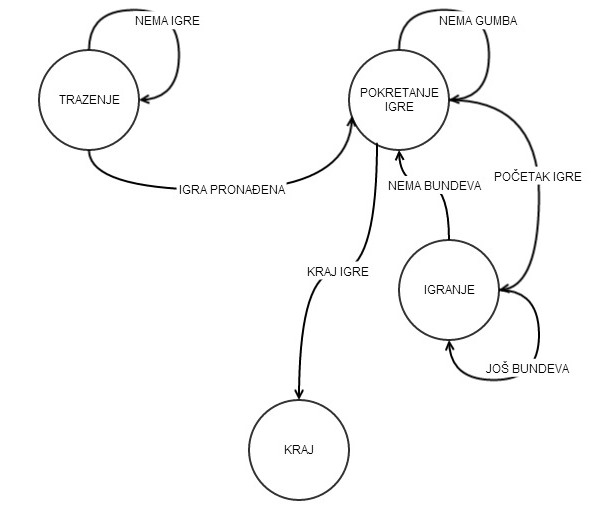
\includegraphics[width=1\textwidth]{model.png}
\caption{Model konačnog automata (Lorena Tomić, 2014.)}
\label{slika-1}
\end{figure}
\newpage
Konačni automat ima 4 stanja te definiranje tranzicije iz jednog stanja u drugo. Stanja su TRAZENJE, POKRETANJE IGRE, IGRANJE i KRAJ. Proces započinje pokretanje stanja TRAZENJE koje ako pronađe igru prelazi u stanje POKRETANJE IGRE. Ako ne uspije pronaći igru, stanje traženja se ponavlja. U stanju POKRETANJE IGRE traži se gumb za start. Agent traži gumb sve dok ga ne pronađe, a u trenutku kad ga pronađe prelazi u stanje IGRANJE. Sve dok u igri postoji još protivnika, odnosno bundeva na koje treba kliknuti, stanje igranja će se ponavljati. U trenutku kada bundeva više nema, vraćamo se u stanje POKRETANJE IGRE. Kada je postignut određeni rezultat, odnosno razina igre, prelazi se u stanje KRAJ.

\chapter{Programski k\^{o}d}

Ovo poglavlje prikazuje programski kod agenta koji igra single player igricu Pumpkin Blitz. Na temelju koordinata i RGB vrijednosti pojedinih piksela određuje se položaj igrice te objekti na koje je potrebno kliknuti. Kako bi prijelaz iz jednog u drugo stanje bio moguć, registrirana su različita stanja i tranzicije utvrđene  na grafičkom prikazu konačnog automata na slici (\ref{slika-1}).

U class Igrac nalaze se četiri stanja koja su definirana za konačni automat, traženje, pokretanje igre, igranje i kraj. U class Trazenje pronalazi se igra na ekranu korisnika. Kada je igra pronađena, pomoću exitcodea se prelazi iz stanja traženja u stanje pokretanja igre. U class PokretanjeIgre provjerava se broj pređenih razina, odnosno broj pokušaja te ako je taj broj veći od 1, igra završava. Ako je broj manji od 1, traži se gumb za start igre. Kada je gumb pronađen, pomoću exitcodea se prelazi u stanje igranja. U class Igranje pretražuje se područje igre za definiranim RGB vrijednostima bundeva te se klikom miša na svaku od tih RGB vrijednosti igra igrica. U class Kraj definira se završetak igre, odnosno prekida se proces. U posljednjem dijelu programskog koda definiraju se stanja i tranzicije između tih stanja koristeći FSMbehaviour.
\definecolor{lbcolor}{rgb}{0.9,0.9,0.9}
\lstset{commentstyle=\textit,language=python}
\lstset{backgroundcolor=\color{lbcolor},rulecolor=}
\begin{lstlisting}[frame=tb]{}
#!/usr/bin/env python
import spade
from bot.bot import *
from time import sleep
import sys 
class Igrac( spade.Agent.Agent ):
  class Trazenje( spade.Behaviour.OneShotBehaviour ):
    def _process( self ):
      originDTM = DTM( { (0, 0): (11, 23, 31),(626, 125): (75, 35, 7),
      (595, 378): (19, 59, 7), (74, 452): (214, 128, 4)}) 
      self.myAgent.origin = findDTM( originDTM, 0, 0,
      self.myAgent.sx, self.myAgent.sy )
      if self.myAgent.origin:
	if self.myAgent.origin != (0, 0):
	  setOrigin( self.myAgent.origin )
	print 'Pronasao sam igru'
	self._exitcode = self.myAgent.P_IGRA_PRONADJENA
	sleep( 1 )
      else:
	print 'Ne mogu pronaci igru!'
	sleep( 1 )
	self._exitcode = self.myAgent.P_NEMA_IGRE
    
  class PokretanjeIgre( spade.Behaviour.OneShotBehaviour ):
    def _process( self ):
      if self.myAgent.igranja > 1:
	self._exitcode = self.myAgent.P_KRAJ_IGRE
	return
      print 'Trazim gumb za start...'
      area = getArea( 0, 0, 800, 600 )
      for y in range( 600 ):
	for x in range( 800 ):
	  if area.getpixel( ( x, y ) ) in [ ( 255, 0, 0 ) ]:
	    print 'Gumb pronadjen!'
	    mouseClick( x, y, True )
            self.myAgent.igranja += 1 
	    self._exitcode = self.myAgent.P_POCETAK_IGRE
	    return
      print 'Ne mogu pronaci gumb za start'
      sleep( 1 )
      self._exitcode = self.myAgent.P_NEMA_GUMBA
      
  class Igranje( spade.Behaviour.OneShotBehaviour ):
    def _process( self ):
      print 'Igram...'
      self.myAgent.broj_pokusaja += 1
      area = getArea( 0, 0, 1028, 480 )
      for x in range( 0, 1028, 10 ):
	for y in range( 0, 480, 10 ):
	  if area.getpixel( ( x, y ) ) in [ ( 79, 29, 0 ), ( 108, 51, 0 ),
	  ( 248, 223, 85 ), ( 130, 75, 15 ), ( 245, 159, 8 ),  ( 0, 48, 0 ),
	  ( 63, 118, 0 ) ]: 
	    print 'Pucam!'
	    mouseClick( x, y, True )
	    sleep( 0.05 )
	    self.myAgent.broj_pokusaja = 0
      if self.myAgent.broj_pokusaja > 50:
	self.myAgent.broj_pokusaja = 0
	self._exitcode = self.myAgent.P_NEMA_BUNDEVA
      else:
        self._exitcode = self.myAgent.P_JOS_BUNDEVA
  
  class Kraj( spade.Behaviour.OneShotBehaviour ):
    def _process( self ):
      print 'Igra je gotova!'
      self.myAgent._kill()
  
  def _setup( self ):
    print 'Igra pocinje!'
    self.origin = None
    self.sx, self.sy = getScreenSize()
    self.igranja = 0
    self.broj_pokusaja = 0
    
    self.S_TRAZENJE        = 1
    self.S_POKRETANJE_IGRE = 2
    self.S_IGRANJE         = 3
    self.S_KRAJ            = 4  
    self.P_NEMA_IGRE           = 100
    self.P_IGRA_PRONADJENA     = 101
    self.P_NEMA_GUMBA          = 200
    self.P_KRAJ_IGRE           = 201
    self.P_POCETAK_IGRE        = 202
    self.P_JOS_BUNDEVA         = 300
    self.P_NEMA_BUNDEVA        = 301
    
    p = spade.Behaviour.FSMBehaviour()
    p.registerFirstState( self.Trazenje(), self.S_TRAZENJE )
    p.registerState( self.PokretanjeIgre(), self.S_POKRETANJE_IGRE )
    p.registerState( self.Igranje(), self.S_IGRANJE )
    p.registerLastState( self.Kraj(), self.S_KRAJ ) 
    p.registerTransition( self.S_TRAZENJE, self.S_TRAZENJE, self.P_NEMA_IGRE )
    p.registerTransition( self.S_TRAZENJE, self.S_POKRETANJE_IGRE,
    self.P_IGRA_PRONADJENA )
    p.registerTransition( self.S_POKRETANJE_IGRE, self.S_POKRETANJE_IGRE,
    self.P_NEMA_GUMBA )
    p.registerTransition( self.S_POKRETANJE_IGRE, self.S_IGRANJE,
    self.P_POCETAK_IGRE )
    p.registerTransition( self.S_POKRETANJE_IGRE, self.S_KRAJ, self.P_KRAJ_IGRE ) 
    p.registerTransition(self.S_IGRANJE,self.S_IGRANJE,
    self.P_JOS_BUNDEVA )
    p.registerTransition( self.S_IGRANJE,self.S_POKRETANJE_IGRE,
    self.P_NEMA_BUNDEVA )
    self.addBehaviour( p, None )
    
if __name__ == '__main__':
  a = Igrac( 'igrac@127.0.0.1', 'tajna' )
  a.start()


\end{lstlisting}

\chapter{Prikaz rada aplikacije}
Slika (\ref{slika-6}) prikazuje pokretanje SPADE-a koje je nužno za funkcioniranje agenta koji igra igru. SPADE se pokreće naredbom runspade.py u terminalu.

\begin{figure}[h]
\centering 
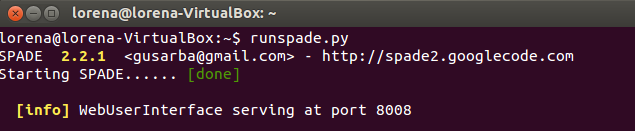
\includegraphics[width=1\textwidth]{spade.png}
\caption{Pokretanje SPADE-a}
\label{slika-6}
\end{figure}

Nakon što je SPADE pokrenut, potrebno je otvoriti web preglednik te igricu Pumpkin Blitz. Slika (\ref{slika-7}) prikazuje izgled navedene igrice.

\begin{figure}[h]
\centering 
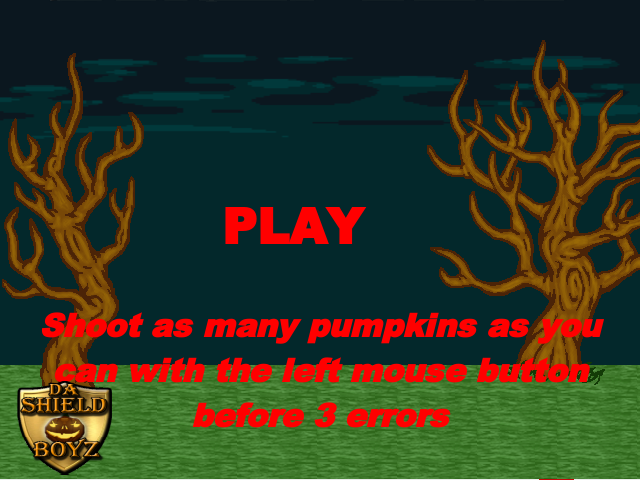
\includegraphics[width=0.75\textwidth]{igra.png}
\caption{Flash igrica Pumpkin Blitz}
\label{slika-7}
\end{figure}

Uz uvjet da je SPADE uspješno pokrenut te da je igra otvorena u web pregledniku, moguće je pokrenuti agenta koji će ju igrati. Agent se pokreće naredbom ./igrac.py. Nakon što je agent pokrenut, na terminalu se ispisuju faze u kojima se proces nalazi. Agent najprije traži igru, zatim gumb za početak razine te u konačnici igra igru. Slika (\ref{slika-8}) prikazuje stanje terminala prilikom pokretanja igre.

\begin{figure}[h]
\centering 
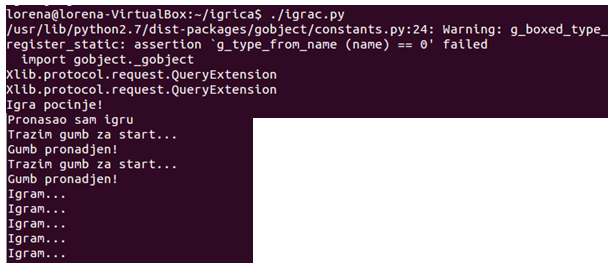
\includegraphics[width=0.80\textwidth]{igranje.png}
\caption{Igranje igre Pumpkin Blitz}
\label{slika-8}
\end{figure}

\chapter{Stručni članci}
\section{CADIA-Player: A General Game Playing Agent}
\emph{Puni naziv i autor članka: Brian Mac Namee, CADIA-Player: A General Game Playing Agent} \citep{FinnsonH2007}
\newline
Mnogi od agenata koji igraju igrice mogu pobijediti većinu, pa i sve ljudske igrače, ali mogu igrati samo igre za koje su programirane. Za razliku od ljudi, agenti su ograničeni na određenu igru i nemaju mogućnost igranja drugih igri. Članak prikazuje implementaciju agenta i poboljšanja efektivnosti simulacija.
Cilj GGP-a (General Game Playing) je osmisliti agente koji uče kako igrati različite igre na temelju pravila određene igre i bez ljudske intervencije. Agenti tako uče strategiju bez da im je to znanje usađeno od strane programera. CADIA igrač koristi pristup simulacije kako bi usmjeravao svoje akcije. Agent korisni Monte Carlo UCT metodu kao osnovnu proceduru pretraživanja te je njegova efikasnost dokazana osvajanjem trećeg godišnjeg GGP natjecanja.
Glavni doprinosi ove teze su \citep{FinnsonH2007}:
\begin{itemize}
  \item Pokazivanje efektivnosti simulacijskog pristupa u kontekstu GGP-a
  \item Razvoj kvalitetnog GGP agenta
  \item Empirijska evaluacija UCT algoritma na širokom spektru igrica
  \item Uvođenje novih tehnika za daljnji razvoj UCT simulacija u novim područjima igara 
   \ldots
\end{itemize}


U tri poglavlja opisuje se pozadinska logika, implementacija CADIA  agenta te algoritmi korišteni za realizaciju agenta.

\subsection{Umjetna inteligencija i igranje igara}
Glavna metoda za primjenu umjetne inteligencije u igranju igara je heurističko pretraživanje, odnosno metoda koja koristi evaluaciju sukladno znanju o igri (npr. figure u šahu) te dodjeljuje heurističku vrijednost pozicijama ovisno o tome koliko su dobre. Postoji veliki broj takvih metoda za single player igrice, dok se za two player igrice heuristički pristup uglavnom bazira na MiniMax algoritmu. Sukladno velikom broju i vrstama igrica, postoji veliki broj algoritama i metoda prikladnih za svaku od njih.

\subsection{MiniMax}
MiniMax je metoda heurističkog pretraživanja za različite igre centrirana oko jednostavne pretpostavke da će protivnik pokušati minimizirati dobit suprotnog igrača koji ju istovremeno nastoji maksimizirati. Stvarna dobit određenog poteza ograničena je minimalnom vrijednosti koju protivnik može odabrati. Slika (\ref{slika-2}) prikazuje game tree s izračunatim maksimalnim vrijednostima. Kvadrati predstavljaju jednog igrača, dok krugovi predstavljaju njegovog protivnika, odnosno redoslijed igranja. Kvadrati na dnu predstavljaju listove i njihova vrijednost je jednaka onome što vraća evaluacijska funkcija. Primjer evaluacijske funkcije u igri na ploču (dama) bi razmatrala razliku u broju figura između dva igrača te tako organizirati pretraživanje da preferira situaciju u kojoj igrač ima više figura od protivnika. Na prvoj razini, odnosno na listovima na lijevoj strani drveta nalaze se dva kvadrata s brojevima 7 i 5. Kada je protivnikov red za igranje, prilikom prelaska u neki od listova, on će uvijek nastojati umanjiti dostupne vrijednosti i odabrati odlazak u list s brojem 5 zbog čega kružni čvor koji spaja ta dva lista poprima vrijednost 5. Kružni čvor označava da je red na prvog igrača koji želi maksimizirati svoju dobit te ima mogućnost odabira između 1 i 5. Igrač odabire vrijednost 5, što je vidljivo i na slici. Sve vrijednosti računaju se sukladno tim pravilima za minimiziranje i maksimiziranje vrijednosti.

\begin{figure}[h]
\centering 
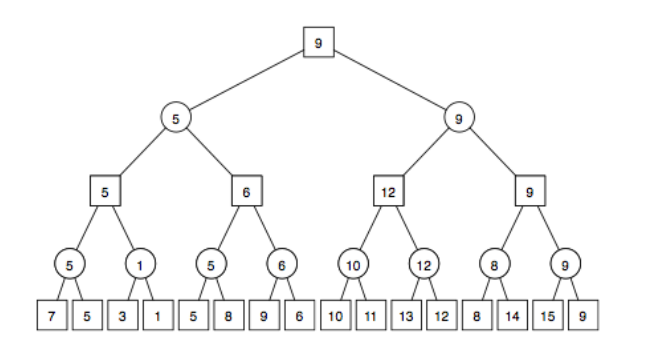
\includegraphics[width=0.95\textwidth]{minimax.png}
\caption{Model konačnog automata \citep{FinnsonH2007}}
\label{slika-2}
\end{figure}
MiniMax je metoda koja je dobra u teoriji, ali je prespora kako bi se koristila u praksi u kompetitivnim programima. Jedan od najefikasnijih dodataka toj metodi je Alpha-Beta Pruning. Metoda omogućava skraćivanje drveta te omogućava dubinsku pretragu.

\subsection{Monte Carlo}
Monte Carlo metode su  vrsta metodi za pojačano učenje. One uče iz iskustva te stoga nemaju potrebe za prethodnim znanjem zadatka koji obavljaju. Prilikom igranja igrica, nije efektivno učiti iz stvarnih iskustava jer učenje dobrih strategija može trajati stotine igara, čak i za čovjeka. Ako Monte Carlo metoda ima internu reprezentaciju zadatka, iskustvo može biti stečeno simulacijom velikog broja igara u vremenu između poteza u stvarnim igrama. Idući potez u igri odabire se sukladno iskustvu stečenom iz simulacija.
\subsection{CADIA-Player}
„Ljudska bića, koja imaju jedinstvenu sposobnost učenja iz iskustava drugih, su isto tako izvanredna za svoju vidljivu nenaklonost tome.“ Douglas Adams (1952-2001), Last Chance to See.
CADIA-Player dobio je ime prema istraživačkom laboratoriju u Reykjavik Sveučilištu, Centru za analizu i dizajn inteligentnih agenata. Player je kreiran kako bi sudjelovao u godišnjem natjecanju GGP organiziranog od strane Stanford Logic Gruoup. Agent koji se natječe na GGP natjecanju mora imati minimalno tri komponente: HTTP server da komunicira sa ostalim igračima, sposobnost razmišljanja korištenjem GDL-a (Game Description Language) te umjetnu inteligenciju i mogućnost igranja igrica koje mu se zadaju. CADIA-Player je napisan u C++ jeziku na Linux/Unix platformi te može biti pokrenut na oba sustava bez izmjena.
CADIA-Player nije ograničen korištenjem samo jednog algoritma pretraživanja. Ima mogućnost odabira  između dva različita algoritma, jedan za single-player igre, a drugi za igre s više igrača. Kao svoj osnovni algoritam pretraživanja, CADIA-Player koristi UCT algoritma koji je varijacija Upper Confidence Bounds algoritma.
Slika (\ref{slika-3}) prikazuje arhitekturu CADIA-Playera. Na vrhu arhitekture nalazi se HTTP server koji pokreće ostatak sustava kao proces dijete. Svaki put kada se igra pokrene, novi proces se pokreće, a stari prekida. Arhitektura se može podijeliti u tri konceptualna sloja prikazana na slici (\ref{slika-3}).
\begin{figure}[h]
\centering 
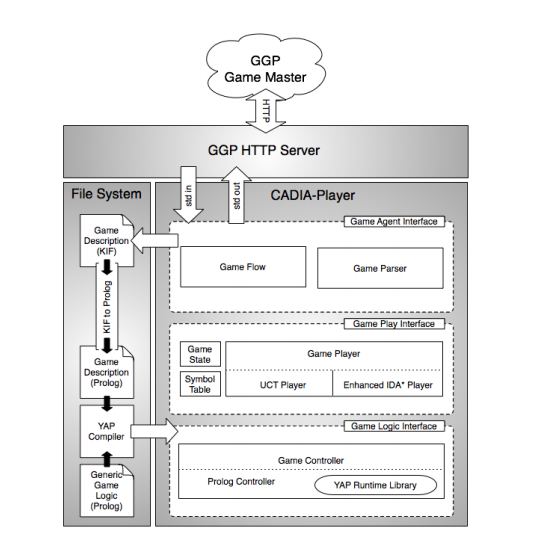
\includegraphics[width=0.80\textwidth]{cadia.png}
\caption{Arhitektura CADIA-Playera \citep{FinnsonH2007}}
\label{slika-3}
\end{figure}

Igra započinje kada GGP HTTP server zaprimi poruku od GM-a da započinje nova igra. Server pokreće novi CADIA-Player proces, izvlači sadržaj HTTP zahtjeva (GM poruka igraču) te ga prosljeđuje procesu. Nakon toga čeka na odgovor od strane procesa prije nego odgovori na HTTP zahtjev. Na drugoj strani, Game Agent Interface čeka na poruku i šalje ju u Game Flow koji ju prepoznaje kao najavu nove igre. Opis igre šalje se u Game Parser koji pokreće Game Play Interface s podatcima iz opisa te ga šalje natrag u Game Flow. Game Flow potom odabire vrstu GameControllera za korištenje. CADIA-Player koristi Prolog Controller  koji koristi Prolog YAP.  Kada se kontroler pokrene, on pronalazi opis igre te ga pokreće eksternim programom koji pretvara KIF u Prolog kod i sprema ga u novu datoteku. Kod se kompajlira te se nastavlja proces pokretanja igre.
Nakon što CADIA-Player najavi da je spreman, može se očekivati novi HTTP zahtjev, ovaj put o potezu igrača. Poruka se šalje i završava  u Game Flowu te šalje upit Game Playeru za odluku o potezu. Game Player donosi odluku koristeći Game Play Interface u koje je uključen kako bi dobio informacije o igri. Kada se odluka postigne, vraća se u Game Flow koji ju šalje  preko HTTP servera natrag ka GM.
Međutim, postoji razlika između prvog poteza i ostatka igre. Nakon prvog poteza, svi zahtjevi za potezom sadrže listu prethodnih poteza svih igrača. Kad je igra gotova, šalje se posebni stop signal i listu posljednjih poteza. Game Logic Interface odgovara na upit o finalnim rezultatima igrača. \citep{FinnsonH2007}

\section{Proactive Persistent Agents}
\emph{Puni naziv i autor članka: Hilmar Finnsson, Proactive Persistent Agents: Using Situational Intelligence to Create Support Characters in Character-Centric Computer Games} \citep{NameeB2004}
\newline
Jednu od najprofitabilnijih računalnih igara u 2002. godini, Metal Gear Solid 2: Sons of Liberty razvijalo je više od 70 ljudi tijekom više od dvije godine s troškom od otprilike 10 milijuna eura. Razvojni tim uključivao je programere, umjetnike i animatore, fizičare, stručnjake za umjetnu inteligenciju, glazbenike i naratore. Igrica je prodana u 2.5 milijuna kopija diljem svijeta. Razvoj računalnih igara u današnje vrijeme predstavlja ozbiljan posao zbog činjenice da je ta industrija financijski veća od filmske industrije. Najveći izazov za umjetnu inteligenciju u računalnim igrama predstavljali su Non-Player Characters (NPCs), likovi upravljani računalom kako bi se popunio svijet igre. Umjetna inteligencija zanemarivala se u mnogo igrica, ali neke poput Simsa i Black and White su pokazale kako kvalitetna umjetna inteligencija može doprinijeti uspješnosti igre.
Člana obrađuje tematiku razvoja inteligentnog agenta koji će određivati ponašanje NPCa u modernim računalnim igrama. Razvoj agenta koji bi upravljao likovima u različitim modernim igrama je nerealno te se usredotočuje na razvoj agenta za support likove u character-centric igrama. Ti likovi poprimaju pozadinske uloge u igrama, igraju uloge kao što su trgovci, barmeni, policija i važni su za stvaranje svijeta računalne igre. Umjetna inteligencija iznimno je važna u takvoj vrsti igara. Arhitektura agenta dozvoljava prilagođavanje različitim situacijama te sudjelovanje likova u naprednim socijalnim interakcijama.

Istraživanje doprinosi području umjetne inteligencije kroz nekoliko elemenata \citep{NameeB2004}:
\begin{itemize}
  \item Kreiranje inteligentnog agenta koji je specifično dizajniran za kreiranje računalno kontroliranih pozadinskih likova u character-centric igrama
  \item Korištenje situacijske inteligencije u igrama, što je do ovog članka jedinstveno
  \item Razvoj sustava, baziranog na fuzzy kognitivnim mapama koji može služiti za upravljanje ponašanjem likova u simulacijama
  \item Razvoj procesa koji omogućava da NPC mijenja svoje ponašanje ovisno o različitim situacijama unutar iste simulacije
  \item Razvoj sustava koji koristi psihološke modele za simuliranje sofisticiranih socijalnih interakcija
  \item Korištenje evaluacijske sheme, najviše radi evaluacije inteligentnih agenata korištenih u igrama te simulacijama virtualnih ljudi
   \ldots
\end{itemize}
Sukladno različitim žanrovima računalnih igara predložene su različite uloge umjetne inteligencije \citep{NameeB2004}:
\begin{itemize}
\item Taktički protivnik
\item Strateški protivnik
\item Partner
\item Support lik
\item Polu-autonomne jedinice
\item Komentatori i sustavi kamera
\item Direktori priče
\end{itemize}
Umjetna inteligencija znatno je povećala kvalitetu i efikasnost igara, no određeni razlozi sprječavaju korištenje sofisticiranih agenata. Neki od tih razloga su \citep{NameeB2004}:
\begin{itemize}
\item Nedostatak CPU resursa potrebnih za umjetnu inteligenciju
\item Nedostatak razvojnog vremena za umjetnu inteligenciju
\item Grafička istraživanja nadjačavaju sve ostalo
\item Sumnja među programerima o nedeterminističkim tehnikama
\item Nedostatak razumijevanja sofisticiranih tehnologija umjetne inteligencije unutar igara
\end{itemize}
Neka od područja koja su znatno poboljšala svijet igara su bila automatsko pronalaženje puta, gdje su se likovi mogli samostalno kretati unutar igre. Kako bi se kreirao efikasan sustav korišteni su mnogi algoritmi i metode, a jedna od najpoznatijih je stroj stanja. To je jednostavni sustav u kojem je konačni broj stanja povezan tranzicijama. Jedan stroj stanja prikazan je na sljedećoj slici (\ref{slika-4}).

\begin{figure}[h]
\centering 
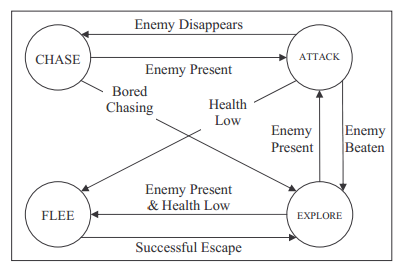
\includegraphics[width=0.50\textwidth]{stroj.png}
\caption{Stroj stanja \citep{NameeB2004}}
\label{slika-4}
\end{figure}

Kako bi se svi podatci pohranili te se znanje očuvalo, koriste se ekspertni sustavi i sustavi za učenje koji koriste razne metode pohrane i pretraživanja podataka.
Iako je istraživanje umjetne inteligencije u akademske svrhe donedavno bilo zanemareno, u današnje vrijeme sve se više i više ulaže u to područje. Osnovane su istraživačke skupine, a određena sveučilišta nude programe za razvoj umjetne inteligencije u igrama. Prilikom istraživanja dolazi do određenih problema zbog nedostatka informacija ili literature te zbog slabe razvijenosti tog područja. Međutim, akademski pristup umjetnoj inteligenciji u igrama postepeno se razvija te igre više nisu bazirane samo na grafici već zahtijevaju određenu mjeru umjetne inteligencije.

\subsection{Inteligentni agenti}
Najveća primjena umjetne inteligencije u računalnim igrama su NPC likovi, a najjednostavniji način da se ta inteligencija implementira su inteligentni agenti. Agent promatra svoju okolinu koristeći određene senzore te prilagođava svoje ponašanje okolini. Agent treba imati sljedeća svojstva \citep{NameeB2004}:
\begin{itemize}
\item Autonomija
\item Sposobnost socijalizacije
\item Proaktivnost
\end{itemize}

Agente se može kategorizirati sukladno različitim kriterijima, a jedan od tih kriterija je njihova implementacija. S obzirom na implementaciju, oni mogu biti \citep{NameeB2004}:
\begin{itemize}
\item Reaktivni (Trenutno stanje svijeta pokreće akciju )
\item Savjetodavni (Trenutno stanje svijeta i željeno stanje generiraju plan)
\item Hibridni
\end{itemize}

\subsection{Proaktivna dosljedna arhitektura agenta}
PPA (Proactive Persistent Agent) arhitektura je razvijena za kontroliranje NPC likova u računalnim igrama. Iako danas postoji mnoštvo igara sa NPC likovima, oni većinom nisu izmodelirani do trenutka kada igrač ne stigne na lokaciju. Kada igrač dođe na lokaciju, NPC čeka njegovu interakciju ili odrađuje određenu predviđenu aktivnost. Ovim člankom nastoji se prijeći preko prepreka korištenjem likova koji su proaktivni i dosljedni. Takvi likovi mogu djelovati ovisno o svojoj volji, odnosno prema svojim ciljevima i motivima. Neovisno o lokaciji igrača, NPC je prisutan u svijetu igre cijelo vrijeme.
Kako bi se razvili ti agenti, kreirana je arhitektura prikazana na sljedećoj slici (\ref{slika-5}).
\begin{figure}[h]
\centering 
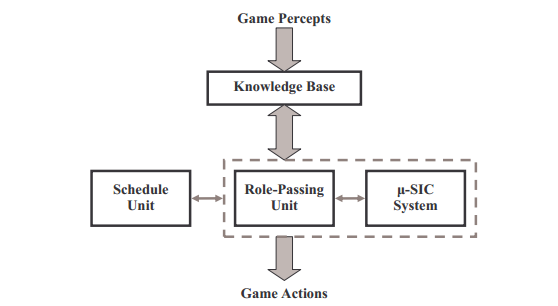
\includegraphics[width=0.90\textwidth]{ppa.png}
\caption{PPA arhitektura \citep{NameeB2004}}
\label{slika-5}
\end{figure}
\newpage

Schedule unit – NPC mora dati dojam postojanja života izvan interakcije s igračem, odnosno NPC ima raspored ponašanja i obaveza
\newline
The Role-Passing Unit – omogućava da se NPC ponaša uvjerljivo u različitim situacijama
\newline
µ-SIC System – omogućava pokretanje interakcije s igračima i drugim NPC likovima u određenim situacijama
\newline 
Knowledge Base – omogućava agentima spremanje informacija o događajima kojima su svjedočili unutar svijeta igre ili što su saznali od drugih NPC likova
\newline
PPA arhitektura razvijena je kako bi se omogućilo kreiranje sofisticiranih, uvjerljivih i aktivnih agenata koji moraju imati sljedeće sposobnosti \citep{NameeB2004}:
\begin{itemize}
\item Prikazivanje uvjerljivih ponašanja
\item Uvjerljivo ponašanje u različitim situacijama
\item Sofisticirane socijalne interakcije
\end{itemize}

PPA to omogućava kroz tri komponente, the schedule unit, the role-passing unit i µ-SIC system.

\subsection{Impementacija}
Mnogi developeri smatraju razvoj računalnih igara kao dva odvojena zadatka: kreiranje tehnologija koje će pokretati igru i stvaranje stvarnog sadržaja igre. Kada se zadatci podijele, developeri razvijaju game-engine, dok dizajneri kreiraju sadržaj igre koji se kasnije učitava u game-engine. PPA arhitektura implementirana je radi promoviranja te ideje te radi što bezbolnije integracije u postojeće igre. Testiranje PPA agenta provelo se u adventure igri te u igri s 3D virtualnim ljudima. Dokazano je da se mogu kreirati likovi koji će se ponašati sofisticirano i uvjerljivo u različitim situacijama.

\chapter{Zaključak}
U ovom projektu prikazan je proces kreiranja proaktivnog agenta koji igra single player igricu. Umjetna inteligencija omogućila je kreiranje strojeva i programa koji obavljaju funkcije koje zahtijevaju inteligenciju. Razvoj tog područja omogućio je izradu agenata koji mogu samostalno obavljati različite funkcije. Ovisno o vrsti agenta, on ima različite mogućnosti i karakteristike. Agent koji igra single player igricu je proaktivan, odnosno on pokazuje ponašanje orijentirano na ostvarenje određenog cilja. Kako bi se bolje prikazao agent koji je kreiran, izrađen je model konačnog automata, odnosno model stanja koji prikazuje sva moguća stanja i tranzicije između tih stanja. Programski kod napisan je u pythonu te je stoga poprilično kratak i jednostavan. U različitim dijelovima koda prolazi se kroz sva četiri definirana stanja kako bi se došlo do konačnog rezultata, odnosno kraja igre. Implementacija agenta zahtijevala je SPADE platformu koja omogućava naprednu opciju FSM behaviour.
\newline
U prvom stručnom članku prikazan je pojam i arhitektura CADIA-Playera napisanog u C++ jeziku. Uz CADIA-Player prikazane su i pojedine metode koje se koriste pri razvoju inteligentnih agenata te njihove karakteristike i doprinosi. Drugi stručni članak govori o proaktivnoj strukturi agenata, odnosno PPA (Proactive Persistent Agent) arhitekturi. Prikazane su karakteristike, sposobnosti te implementacija navedene arhitekture te objašnjen njen doprinos primjeni umjetne inteligencije u računalnim igrama. 

\addcontentsline{toc}{chapter}{Bibliografija}
\bibliography{foi.bib}
\end{document}
